% Latex template: mahmoud.s.fahmy@students.kasralainy.edu.eg
% For more details: https://www.sharelatex.com/learn/Beamer

\documentclass{beamer}					% Document class
\geometry{papersize={15cm,10cm}}

\setbeamertemplate{footline}[text line]{%
  \parbox{\linewidth}{\vspace*{-8pt}Probing phase transitions of DNA-protein condensates using single molecule localization microscopy\hfill\insertshortauthor\hfill\insertpagenumber}}
\setbeamertemplate{navigation symbols}{}

\usepackage[english]{babel}				% Set language
\usepackage[utf8x]{inputenc}			% Set encoding

\mode<presentation>						% Set options
{
  \usetheme{default}					% Set theme
  \usecolortheme{default} 				% Set colors
  \usefonttheme{default}  				% Set font theme
  \setbeamertemplate{caption}[numbered]	% Set caption to be numbered
}

% Uncomment this to have the outline at the beginning of each section highlighted.
%\AtBeginSection[]
%{
%  \begin{frame}{Outline}
%    \tableofcontents[currentsection]
%  \end{frame}
\usepackage{graphicx}					% For including figures
\usepackage{booktabs}					% For table rules
\usepackage{hyperref}	
\usepackage{tikz-network}				% For cross-referencing
\usepackage[absolute,overlay]{textpos}
\usepackage{bm}
\usepackage[font=small,labelfont=bf]{caption}				% For cross-referencing

\title{Probing phase transitions of DNA-protein condensates using single molecule localization microscopy}	% Presentation title
\author{Clayton W. Seitz}								% Presentation author
\date{\today}									% Today's date	

\begin{document}

% Title page
% This page includes the informations defined earlier including title, author/s, affiliation/s and the date
\begin{frame}
  \titlepage
\end{frame}


% The following is the most frequently used slide types in beamer
% The slide structure is as follows:
%
%\begin{frame}{<slide-title>}
%	<content>
%\end{frame}


\begin{frame}{Outline}
\begin{itemize}
\item Introduction: biological motivation and broad overview of microscopy approaches, IDRs of BRD4/MED1
\item Methods: High-throughput and super-resolution imaging, PSF engineering, dSTORM chemistry, photoswitching dynamics
\item Methods: Motivation for deep learning methods for 3D imaging at high density
\item Methods: Bayesian clustering algorithms on high density data
\item Results: Induction of gene expression, colocalization with phase separation markers
\item Results: Statistics of nucleosome organization in phase separated clusters
\end{itemize}
\end{frame}

\begin{frame}{A phase separation model for transcriptional control}
IDRs of BRD4/MED1
\end{frame}

\begin{frame}{The role of nucleosome organization in phase separation of DNA-protein condensates}
HaloTag labeling method
\end{frame}

\begin{frame}{Single molecule localization microscopy for super-resolution}
Direct stochastic optical reconstruction microscopy
Fourier shell correlation
\end{frame}


\begin{frame}{Statistics of sCMOS cameras}
\end{frame}

\begin{frame}{Point spread function engineering for three-dimensional imaging}
\end{frame}

\begin{frame}{Localization microscopy as statistical inference}
\end{frame}


\begin{frame}{Localization microscopy as statistical inference}
\end{frame}

\begin{frame}{Photoswitching dynamics are a major determinant of localization precision}
\end{frame}

\begin{frame}{A deep learning framework for localization microscopy}
Deep learning performs better than maximum likelihood estimators
\end{frame}

\begin{frame}{A deep learning framework for localization microscopy}
\end{frame}

\begin{frame}{Bayesian clustering algorithms on high density data}
Bayesian nonparametrics in general
\end{frame}

\begin{frame}{Bayesian clustering algorithms on high density data}
Bayesian nonparametrics
\end{frame}

\begin{frame}{Inducing GBP5 gene expression with Inteferon-$\gamma$}
\begin{figure}
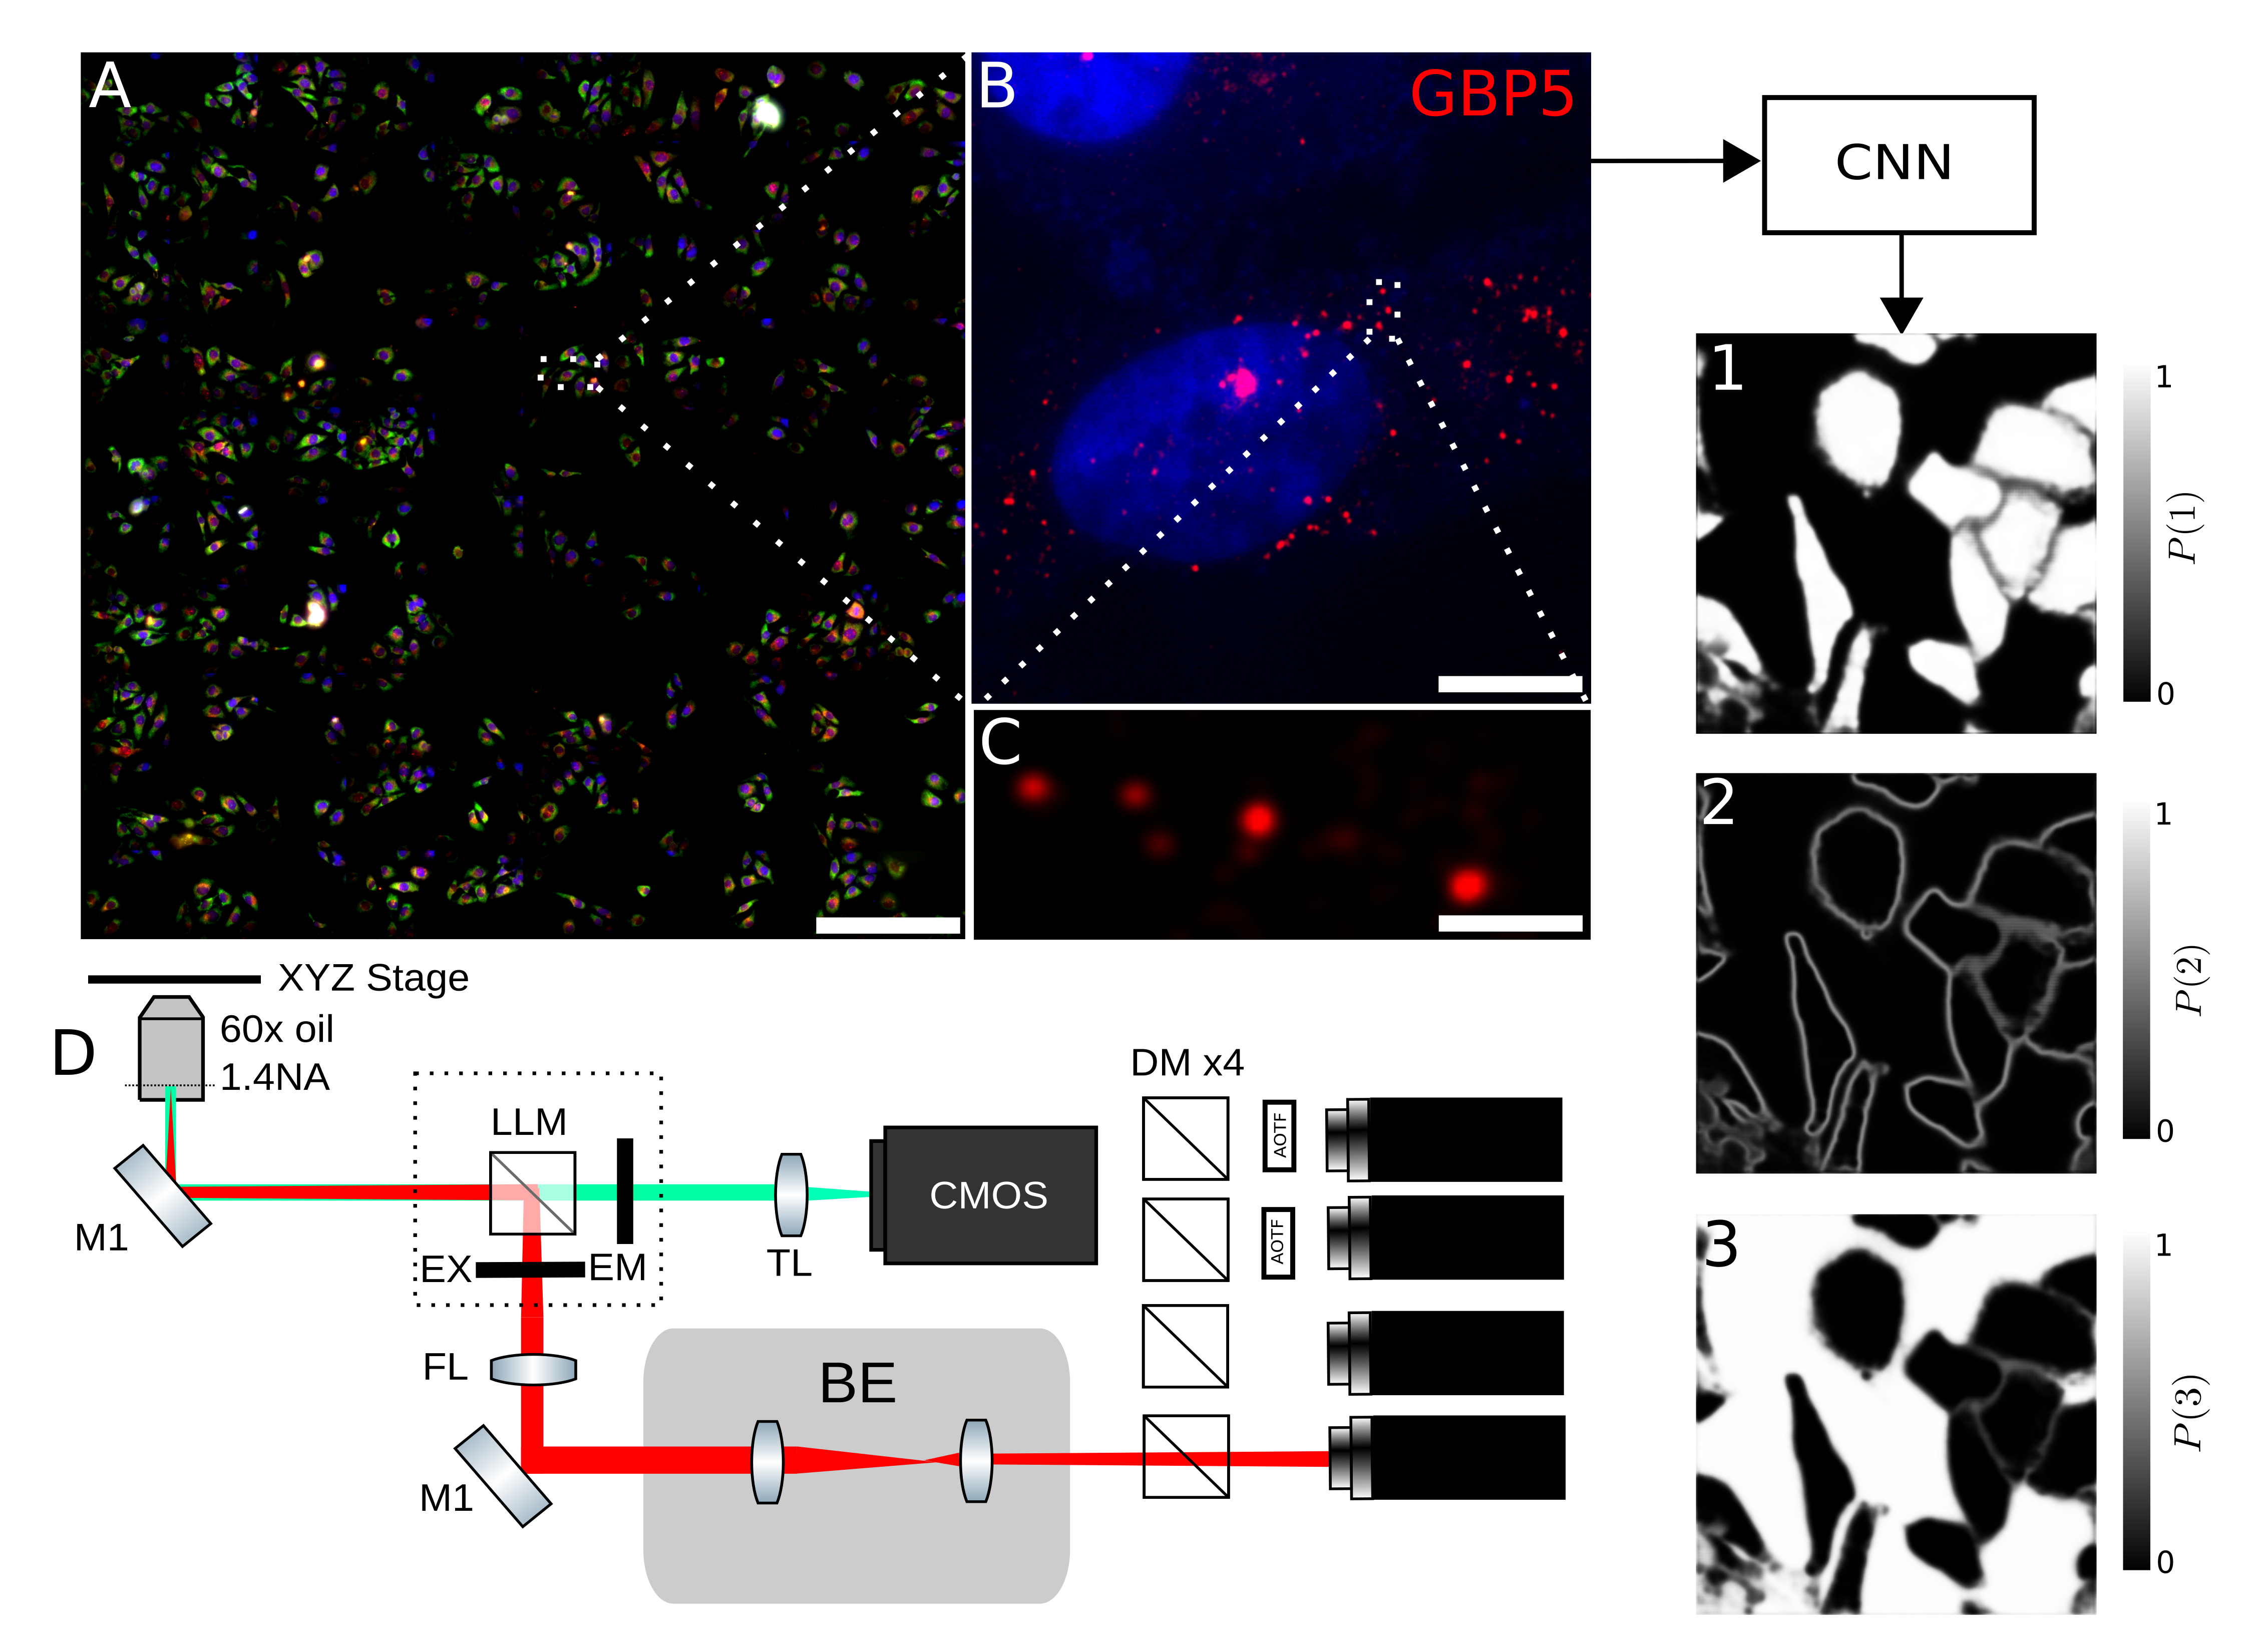
\includegraphics[width=11.5cm]{Figure-1.png}
\end{figure}
\end{frame}

\begin{frame}{Colocalization of nascent GBP5 mRNA with phase separation markers}
\begin{figure}
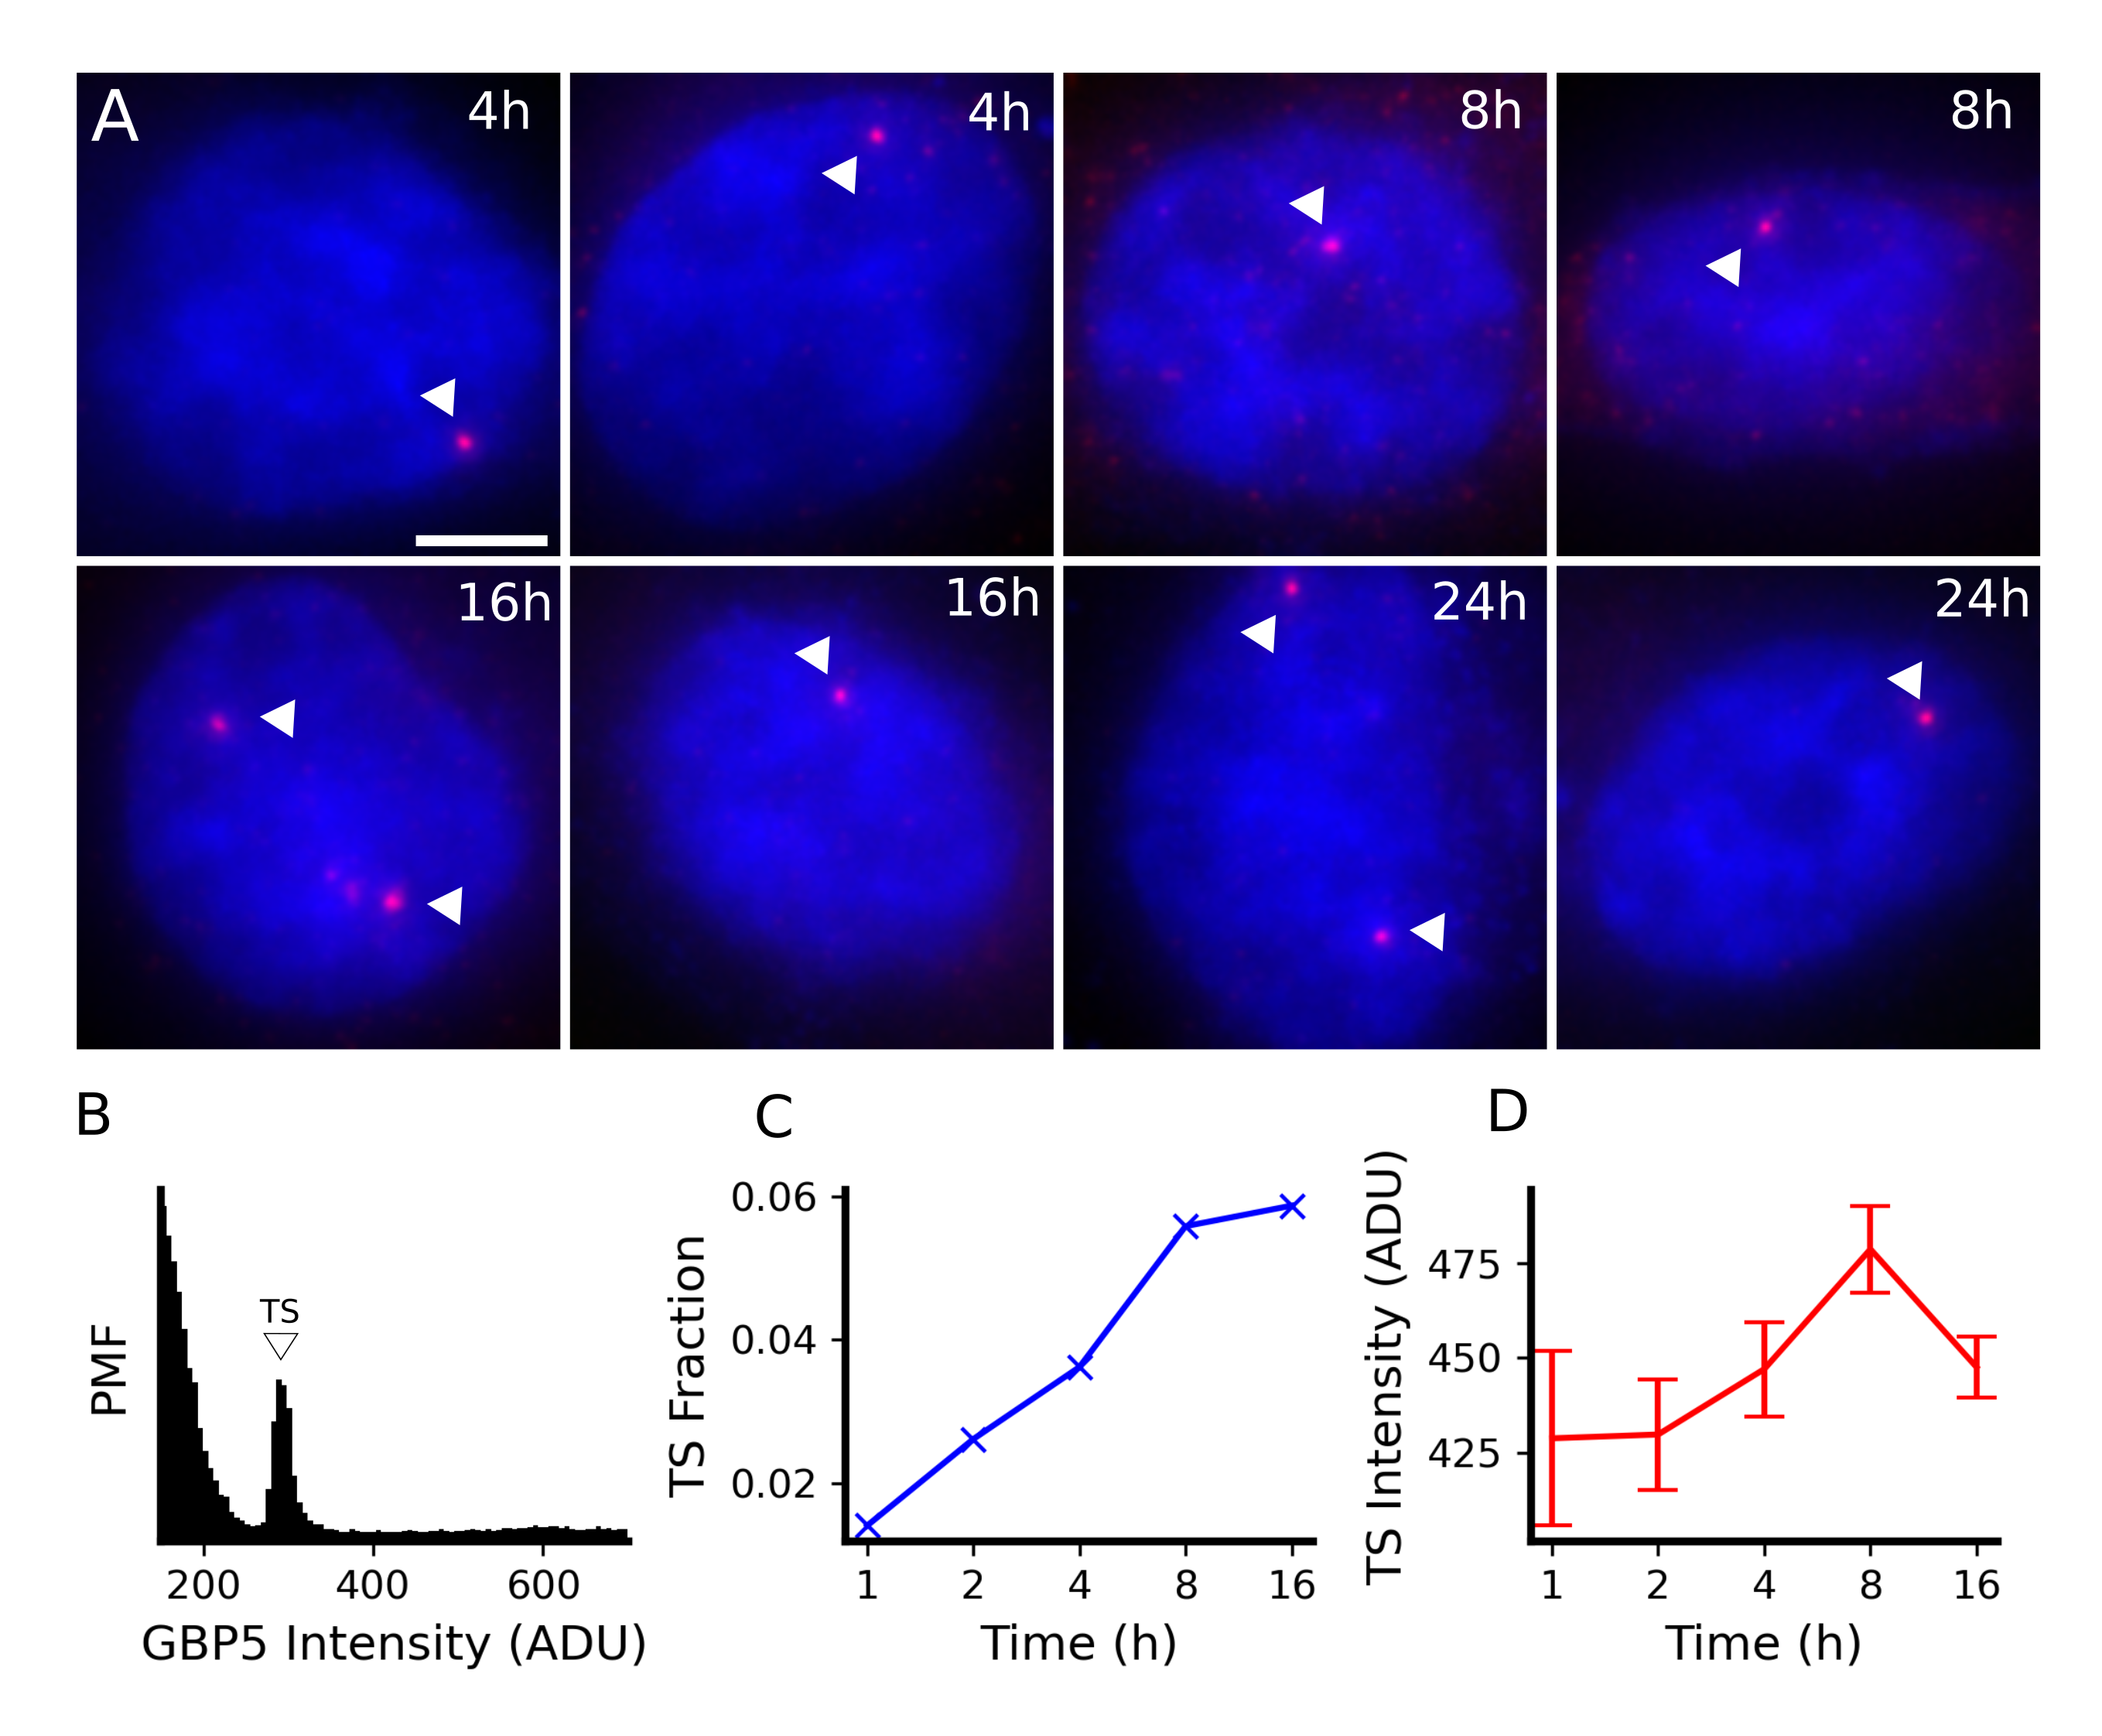
\includegraphics[width=10.5cm]{Figure-2.png}
\end{figure}
\end{frame}

\begin{frame}{Colocalization of nascent GBP5 mRNA with phase separation markers}
\begin{figure}
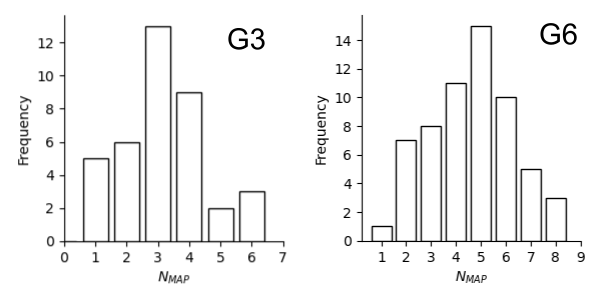
\includegraphics[width=10cm]{Figure-5.png}
\end{figure}
\end{frame}

\begin{frame}{Costaining of H2B/BRD4/MED1 in interphase Hela cells}
\end{frame}

\begin{frame}{Cluster analysis of H2B at putative transcriptional condensates}
\end{frame}

\begin{frame}{Physical cluster analysis of H2B at putative transcriptional condensates}
\end{frame}

\end{document}